% Gemini theme
% https://github.com/anishathalye/gemini
%
% We try to keep this Overleaf template in sync with the canonical source on
% GitHub, but it's recommended that you obtain the template directly from
% GitHub to ensure that you are using the latest version.

\documentclass[final]{beamer}

% ====================
% Packages
% ====================

\usepackage{amsmath, amsthm, amssymb, amsfonts}
\usepackage[size=custom,width=120,height=72,scale=1.0]{beamerposter}
\usetheme{gemini}
\usecolortheme{gemini}
\usepackage{bigints}
\usepackage{booktabs}
\usepackage{epigraph}
\usepackage{float}
\usepackage[T1]{fontenc}
\usepackage{graphicx}
\graphicspath{ {./img/} }
\usepackage{hhline}
\usepackage{hyperref}
\hypersetup{
colorlinks=true,
linkcolor=cyan,    
urlcolor=magenta,
pdftitle={Loop Classical Mechanics},
}
\usepackage{lmodern}
\usepackage{mathrsfs}
\usepackage{mathtools}
\usepackage{pgfplots}
\pgfplotsset{compat=1.14}
\usepackage{soul}
\usepackage{tcolorbox}
\usepackage{tikz}
\usepackage{tikz-cd}
\usepackage[normalem]{ulem}

\newenvironment{highlight}
{\begin{tcolorbox}[colback=lightblue, boxrule=0pt, frame empty]}
{\end{tcolorbox}}

% ====================
% Lengths
% ====================

% If you have N columns, choose \sepwidth and \colwidth such that
% (N+1)*\sepwidth + N*\colwidth = \paperwidth
\newlength{\sepwidth}
\newlength{\colwidth}
\setlength{\sepwidth}{0.025\paperwidth}
\setlength{\colwidth}{0.3\paperwidth}

\setlength\epigraphwidth{\colwidth}

\newcommand{\separatorcolumn}{\begin{column}{\sepwidth}\end{column}}

\newcommand{\bs}{\backslash}
\newcommand{\ca}{\cancel}
\newcommand{\dis}{\displaystyle}
\newcommand{\ex}{\exists \:}
\newcommand{\fa}{\forall \:}
\newcommand{\im}{\text{im}}
\newcommand{\mb}{\mathbb}
\newcommand{\mc}{\mathcal}
\newcommand{\mf}{\mathfrak}
\newcommand{\preim}{\text{preim}}
\newcommand{\ra}{\rightarrow}
\newcommand{\sing}{\text{Sing}}

\newcommand{\inc}[1]{\xhookrightarrow{#1}}
\newcommand{\mor}[1]{\xrightarrow{#1}}
\newcommand{\lmor}[1]{\xrightarrow[#1]}

\theoremstyle{remark}
\newtheorem*{remark}{Remark}

% ====================
% Title
% ====================

\title{Loop \sout{Quantum Gravity} Classical Mechanics: Algebraic Topology for Non-holonomic Mechanics}

\author{Siddhartha Bhattacharjee}

\institute[shortinst]{University of Waterloo}

% ====================
% Footer (optional)
% ====================

\footercontent{
Blog (Tempus Spatium): \href{https://booodaness.github.io/tempus-spatium/}{https://booodaness.github.io/tempus-spatium/} \hfill
\href{https://uwaterloo.ca/physics-astronomy/events/phys-10-seminars}{PHYS10} Poster Fair, March 22, 2024 \hfill
\href{mailto:s3bhatta@uwaterloo.ca}{s3bhatta@uwaterloo.ca}}
% (can be left out to remove footer)

% ====================
% Logo (optional)
% ====================

% use this to include logos on the left and/or right side of the header:
% \logoright{\includegraphics[height=7cm]{logo1.pdf}}
% \logoleft{\includegraphics[height=7cm]{logo2.pdf}}

% ====================
% Body
% ====================

\begin{document}

\begin{frame}[t]
\begin{columns}[t]
\separatorcolumn

\begin{column}{\colwidth}

\epigraph{\textit{There is no clear-cut distinction between example and theory.}}{Michael Atiyah}

\begin{block}{$n$-Simpices (\emph{Triangles!})}
The \textbf{standard $n$-simplex} $\Delta^n \subsetneq \mathbb{R}^{n+1}$ is the \emph{convex hull} of the standard basis vectors $\{ e_0, \dots, e_n \}$,

$$\Delta^n = \left\{ \sum_i t_i e_i : \sum_i t_i = 1; t_0, \dots, t_n \geq 0 \right\}$$

$(t_0, \dots, t_n)$ are the \textbf{barycentric coordinates} of $\Delta^n$. Associated with a standard $n$ simplex are its \textbf{face (inclusion) maps} (opposite to the $e_i$) which are \emph{affine linear maps} $\phi^n_i : \Delta^{n-1} \inc{} \Delta^n$ with,

$$\phi^n_i = (e_0, \dots, \widehat{e}_i, \dots, e_n)^\flat : (t_0, \dots, t_{n-1}) \mapsto (t_0, \dots, t_{i-1}, 0, t_i, \dots, t_{n-1})$$

where the widehat denotes the omission of the $i$-th index. The $i$-th \textbf{face} of $\Delta^n$ is the \emph{subsimplex} $\phi^n_i(\Delta^{n-1})$. The boundary of a non-oriented $n$-simplex then consists (up to permutation) the union of all its faces.

Standard $n$-simplices are a well-understood and surprisingly rich class of topological spaces. It is therefore convenient to understand an arbitrary topological space $X$ and its topological invariants via continuous maps from $n$-simplices.
\end{block}

\begin{block}{Singular $n$-simplices (\emph{Curved triangles!})}
A \textbf{singular $n$-simplex in $X$} is a $C^1$ map $\sigma_n : \Delta^n \to X$. The set of all (singular) $n$-simplices in $X$ is denoted as $\sing_n(X)$. Analogous to $n$-simplices, singular $n$-simplices are associated with \textbf{face maps} $d^n_i : \sing_n(X) \to \sing_{n-1}(X), \sigma_n \mapsto \sigma_n^{(i)} = \sigma_n \circ \phi^n_i$ with the $i$-th \textbf{face} of $\sigma_n$ being $d^n_i(\sigma_n) = \sigma_n^{(i)}$.

The above information can be captured as an example commutative diagram,

\begin{figure}[H]
\begin{center}
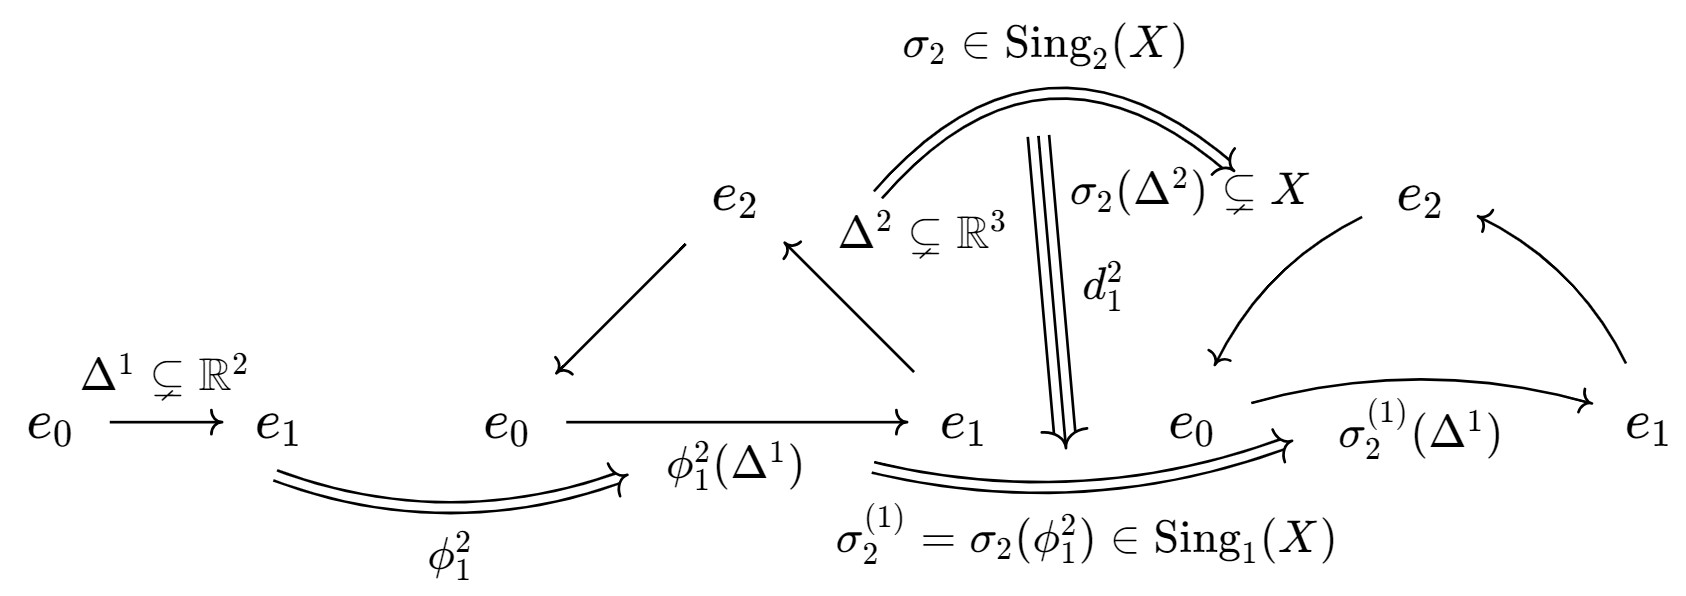
\includegraphics[width=0.75\colwidth]{singular_simplex}
\end{center}
\caption{The standard $1$-simplex $\Delta^1$; face maps $\phi^2_i$ to the standard $2$-simplex $\Delta^2$; and a singular $2$-simplex $\sigma_2$ in $X$.}
\end{figure}

To talk about the boundary of $n$-simplices in $X$, we will need to construct a \emph{free Abelian group} structure on simplices. 
\end{block}

\begin{block}{Singular $n$-chains (\emph{Triangles form modules, yay!})}
The \textbf{singular $n$-chains} of $X$ are members of the \emph{free Abelian group} generated by singular $n$-simplices,

$$S_n(X) = \mathbb{Z} \: \sing_n(X)$$

Therefore, an $n$-chain is a \emph{finite $\mathbb{Z}$-linear combination of simplices}, $\displaystyle{\sum_{i \in I \subsetneq \mathbb{N}} a_i \sigma_i}$ s.t. for all $i \in I$, we have, $a_i \in \mathbb{Z}, \sigma_i \in \sing_n(X)$. This construction is instrumental as $S_n(X)$ behaves as a $\mathbb{Z}$-module. It is \emph{free} in the sense that $\sing_n(X)$ is a $\mathbb{Z}$-basis for it. The \textbf{rank} of $S_n(X)$ is defined to be $\dim(\sing_n(X))$.

\end{block}

\end{column}

\separatorcolumn

\begin{column}{\colwidth}
Now, the \textbf{boundary operator} $\partial_n : \sing_n(X) \to S_{n-1}(X)$ is defined as,

\begin{highlight}
$$\partial_n(\sigma_n) = \sum_{i=0}^n (-1)^n d^n_i(\sigma_n) = \sum_{i=0}^n (-1)^i \sigma_n^{(i)}$$
\end{highlight}

This canonically generates a \emph{homomorphism} between chains, $\partial_n : S_n(X) \to S_{n-1}(X)$ with

$$\partial_n \left( \sum_{k=0}^r a_k \sigma_k \right) = \sum_{k=0}^r a_k \partial_n(\sigma_k)$$

\begin{alertblock}{$n$-cycles and $n$-boundaries (\emph{Loops and surfaces go brrr!})}
An \textbf{$n$-cycle} in $X$ is an $n$-chain $c \in S_n(X)$ with a \emph{vanishing boundary} i.e., $\partial_n c = 0$. The \textbf{group of $n$-cycles} in $X$ is the subset (of $S_n(X)$),

$$Z_n(X) = \ker(\partial_n : S_n(X) \to S_{n-1}(X))$$

Similarly, an \textbf{$n$-dimensional boundary} in $X$ is an $n$-chain $c \in S_n(X)$ s.t. there exists an $(n+1)$-chain $b \in S_{n+1}(X)$ satisfying $\partial_{n+1} b = c$. The \textbf{group of $n$-boundaries} of $X$ is consequently, 

$$B_n(X) = \im(\partial_{n+1} : S_{n+1}(X) \to S_n(X))$$
\end{alertblock}

A celebrated theorem is that boundaries have no boundaries, $\partial_{n} \circ \partial_{n+1} = 0$, which follows from the antisymmetric nature of $\partial$. In other words, boundaries are always cycles, $B_n(X) \subseteq Z_n(X)$. This motivates us to define a \textbf{chain complex}, which is a sequence of graded ($\mathbb{Z}$-indexed) Abelian groups $\{ A_n \}$ together with homomorphisms $\partial_n : A_n \to A_{n-1}$ satisfying $\partial_n \circ \partial_{n+1} = 0$.

The chain complex associated with a topological space $X$ is its \textbf{singular chain complex},

\begin{highlight}
$$... \mor{\partial_{n+1}} S_n(X) \mor{\partial_n} S_{n-1}(X) \mor{\partial_{n-1}} ... \mor{\partial_1} S_0(X) \mor{\partial_0} 0$$
\end{highlight}

\begin{block}{Singular homology (\emph{Cycles with no interior measure holes!!!})}
The $n$-th \textbf{singular homology} group of $X$ is the \emph{quotient group},

\begin{highlight}
$$H_n(X) = \frac{Z_n(X)}{B_n(X)} = \{ [c] : c \in Z_n(X) \} = \{ c + B_n(X) : c \in Z_n(X) \}$$
\end{highlight}

Formally, $H_n(X)$ identifies cycles differing by boundaries i.e. \textbf{homologous} cycles. Therefore, each homology class is represented by a distinct cycle that contains no boundaries --- which are $n$-dimensional holes! Intuitively, homology 'forgets' boundaries to detect topological invariants like holes of a given dimension. For example, let $\sigma_n(\Delta^n) = \partial_{n-1} \sigma_{n-1}(\Delta^{n-1})$. Informally, since $\sigma_n(\Delta^n)$ is a convex region, it can be continuously \emph{contracted} to a point, which is 'uninteresting' from the point of view of detecting holes. This is why modding out by $B_n(X)$ allows us to 'see' cycles that cannot be contracted to inner regions, thereby counting holes.

\begin{figure}[H]
\begin{center}
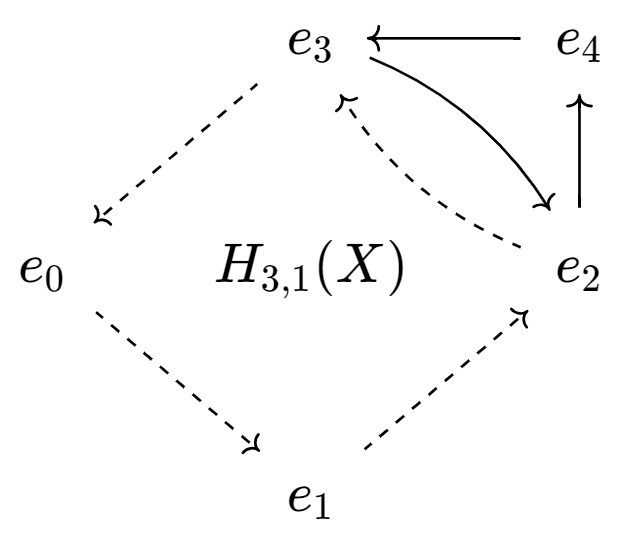
\includegraphics[width=0.3\colwidth]{homology_class}
\end{center}
\caption{A $3$-hole $H_{3, 1}(X)$, represented by the (dotted) non-boundary cycle $(e_0, e_1, e_2, e_3)$. The (undotted) boundary $b=(e_4, e_3, e_2)$ does not affect the hole, so that $H_{3, 1}(X)$ is homologous to the cycle $b + H_{3, 1}(X)$.}
\end{figure}

\end{block}

\end{column}

\separatorcolumn

\begin{column}{\colwidth}

\begin{block}{Homotopy (\emph{Non-Abelianized Loops!})}

Homotopy is a vast discipline so we will only cover it very briefly. A \textbf{$n$-loop} $\gamma$ in a \emph{pointed topological space} X with base $p \in X$ is an $n$-cycle i.e. $\partial_n \gamma = 0$. The \textbf{$n$-loop space} $\mc{L}_n(X)$ is the set of all $n$-loops containing the base i.e., $\mc{L}_n(X) = \{ \gamma \in \sing_n(\mb{R}^{n+1}) : p \in \gamma(\Delta^n), \partial_n \gamma = 0 \}$. We say that two loops $\gamma, \delta \in \mc{L}_n(X)$ are \textbf{homotopic} i.e. $\gamma \sim \delta$ iff there exists a $C^1$ map called a \textbf{homotopy} $h : \Delta^1 \times \Delta^n \to \mc{L}_n(X)$ s.t. $h(e_0, \cdot) = \gamma$ and $h(e_1, \cdot) = \delta$, allowing us to define the \textbf{$n$-th homotopy group} of $X$,

\begin{highlight}
$$\pi_n(X) = \mc{L}_n(X)/\sim$$
\end{highlight}

To complete the notion of a homotopy group, we define the \textbf{concatenation} of $n$-loops as the $\Psi$-composition of the \textbf{wedge sum} of their domains, $x \in \Delta^n \vee \Delta^n \implies (\gamma * \delta)(x) = \sigma_n(\Psi(x))$ where $\Delta^n \vee \Delta^n = \left( \Delta^n \sqcup \Delta^n \right)/\equiv$ with $\Delta^n \sqcup \Delta^n$ being their \textbf{disjoint union} $\Delta^n \times \{ 0 \} \cup \Delta^n \times \{ 1 \}$ and $\equiv$ identifying the faces $\phi^n_n(\Delta^{n-1})$ and $\phi^n_1(\Delta^{n-1})$. Furthermore, $\Psi$ is the map $\Delta^n \vee \Delta^n \to \Delta^n$. Informally, this corresponds to gluing the said faces together. $(\pi_n(X), *)$ are \emph{non-Abelian groups} with the identity element being the \textbf{constant curve} $\gamma_e = \pi_{\{ p \}}$. Finally, a loop $\gamma \in \mc{L}(X)$ is \textbf{contractible} if it is \textbf{null-homotopic} i.e. homotopic to $\gamma_e$.

Therefore, \emph{each non-contractible homotopy class in $\pi_n(X)$ represents a hole with an $n$-dimensional boundary!}

\end{block}

\begin{block}{Holonomies (\emph{States are loop-like, \emph{not} point-like!!!})}

Let $\mu$ be a \textbf{Borel measure} on $X$ i.e. any measure on its \emph{$\sigma$-algebra of Borel sets}, $\mf{B}$ (which is the smallest $\sigma$-algebra on X containing its \emph{open sets}. Let $A$ be, for brevity, a scalar field $X \to \mb{R}$ representing a \textbf{physical observable} with $X$ being the \emph{configuration space} and $\mb{R}$ being the \emph{state space}. Then, the \textbf{holonomy} corresponding to $A$ along an $n$-loop $\gamma \in \mc{L}_n(X)$ is given by the $\mb{Z}$-linear functional,

$$W_A[\gamma] = \bigointsss_{x \in \gamma} d \mu \: A(x)$$

Now, by the Fundamental Theorem of Calculus, the state space $\mc{S}(X)$ corresponding to $p \in X$ is the set of holonomies for all loops based at $p$,

$$\mc{S}(X) = \bigcup_{n = 0}^{\infty} \: \bigcup_{\gamma \in \mc{L}_n(X)} W_A[\gamma]$$

As a result, \textbf{if we forget paths which do not update $A$, the state space is identical to the modded loop space!} This is an unexpected physical consequence of the first isomorphism theorem:

\begin{highlight}
$$\mc{S}(X) \cong_{\text{Set}} \mc{L}(X)/{\ker(W_A)}$$
\end{highlight}

$A$ is said to be \textbf{holonomic} if its holonomy is \emph{trivial} i.e. $\ker(W_A) = \mc{L}(X)$. Then, $\mc{S}(X)$ is the singleton $\{ A(p) \}$, allowing us to use the usual functional treatment to manipulate states. However, in general, $A$ is otherwise i.e. \textbf{non-holonomic}, and the best we can treat states is as sections of the bundle $(S(X), \varphi \circ \pi_{\{ p \}}, \{ p \})$ which is bundle-isomorphic to $\mc{L}(X), \pi_{\{ p \}}, \{ p \})$ where $\varphi : \mc{S}(X) \to \mc{L}(X)$.

\end{block}

\begin{block}{References}

\nocite{*}
\footnotesize{\bibliographystyle{plain}\bibliography{poster}}

\end{block}

\end{column}

\separatorcolumn
\end{columns}
\end{frame}

\end{document}
